\begin{abstract}
 The abstract goes here...
\end{abstract}



%*****************************************************************************
%*****************************************************************************
\chapter{Introduction}
%*****************************************************************************
%*****************************************************************************
Some short information how to get started:
\begin{itemize}
	\item Download the \texttt{tuddesign} files from \url{http://exp1.fkp.physik.tu-darmstadt.de/tuddesign/}, these are required to run any of the KOM templates!
	\item Open the main file of your template document and adjust the section containing the main document information. Afterwards, it might also be a good idea to adjust the filenames to your needs.
	\item For your convenience, common \LaTeX\ examples are included with the template and can be found in the file \texttt{content.tex}.
	\item Carefully check the comments included in the \LaTeX\ sources of the template and the manual of \texttt{tuddesign} (for general problems with \texttt{tuddesign} it is a good idea to visit the forum on their website). General \LaTeX\ problems should be resolved via the web, manuals, or the corresponding usenet groups (\texttt{de.comp.text.tex}, \texttt{comp.text.tex}).
\end{itemize}



%*****************************************************************************
%*****************************************************************************
\chapter{State of the Art}\label{ch:stateOfTheArt}
%*****************************************************************************
%*****************************************************************************
\section{Overview}
In this chapter, the history and the state of the art of pervasive games in general and exergames in special will be presented. Popular representatives like <em>Ingress</em> [33] or <em>Pokémon GO</em> [34], published by Niantic \footnote{\url{https://www.nianticlabs.com/}}, will be looked at.

Additionally, some interesting approaches about vehicle recognition and number plate region detection will be discussed as the concept presented in this thesis also includes automatic vision-based vehicle recognition.

\section{Pervasive Games}
\subsection{Definition}
Although the term pervasive gaming is becoming more and more popular within the last years, its definition is still vague [39]. One is calling them a new type of digital games that combine game reality and physical reality within the gameplay [46].

Another definition says, that it is a game, in which the game world exists beside the everyday environment and that never stops but surrounds the player 24 hours a day [47].
E. Nieuwdorp (TODO name) defined pervasive games as special type of game that emphasizes the relation between reality and game [39].

There is some consensus in those definitions, such as the importance of the relation between the reality and the game world.

But instead of bringing up another definition to compete with the other ones, this thesis compiles definitions of some works to define the boundary of pervasive games, as fitted for this thesis’ scope.

A definition that tries to comprise the bottom line of many other definitions was made by Hock (TODO name): <em>”A pervasive game is an overlay of the real world where it (the overlay) is persistently present. It takes place in physical environments and its gameplay interacts with or is in some way related to parts of the real world. It thereby blurs the boundaries between reality and virtuality. It ideally integrates smoothly into its user’s everyday life where it ideally is omnipresent which means that the user should be able to play it at any time in any place”</em> [26].


\subsection{Beyond Traditional Games}
Montola (TODO name) tried to approach the definition problem by investigating all kinds of games that have been classified as pervasive games for different and not unique reasons. He found out, that there is no single common denominator of those reasons.

But regarding the magic circle of play (see next section TODO), each of these games broke out of this circle in a distinct manner [14].

\subsubsection{The Magic Circle of Play}
Huizinga (TODO name) defines a play as <em>some activities</em> in <em>some places</em> that are considered playfully by the players to belong to the game and not to reality [45].

Traditionally, a game takes place at <em>“certain spaces, at certain times, by certain players”</em> [14]. This is referred to as the magic circle of play.

For a pervasive game, this circle does not have a rigid border but a “permeable membrane where conventional meanings, psychological artefacts and environments, and players alike can slip through” [39].

In relation to the magic circle of play, another definition for a pervasive game is <em>”a game that has one or more salient features that expand the contractual magic circle of play socially, spatially or temporally.”</em> [14]

In the following, each of the named dimensions, in which pervasive games expand the magic circle of play, are described.

\subsubsection{Spatial Expansion}
This means, that the location, where the game can be played at, is unclear or unlimited [14]. Thinking of the example from the beginning of this thesis, that game may have started at a factory site, but the actual spread of the zombies is unclear and could be unlimited.

Montola notes that there are challenges with this kind of expansion, causing people to play the game on unwanted places like hospitals or creating hazardous situations in traffic [14].

\subsubsection{Temporal Expansion}
In classic games, a play session has a well defined start and end time. Pervasive games can break these limits. Not only does the temporal expansion obfuscate the start and end time of a game, it also blurs the border between everyday life and gaming by leaving the player in the dark about if he is playing at the moment or not [14].

<em>”Boring moments of life can be enchanced by any mobile game, but temporal expansion reaches even the moments of not-playing”<em>, because <em>”any action could be a game action”</em> [14].

\subsubsection{Social Expansion}
The social expansion obfuscates the boundary of playership [14]. Thinking back to the example of <em>The Running Dead</em> in the beginning of this thesis, it wasn’t clear who is a participant and who isn’t. A noninvolved person could have watched a persecuted player and could have tried to help him. So the noninvolved person would become a participant without even knowing about it himself.

\subsubsection{Subcategories of Pervasive Games}
There are many subcategories of pervasive games, such as immersive games, serious games or exergames, to name a few. Immersive games combine spatial, temporal and social expansion. In this genre, it’s hard to differentiate games from non-games, because everything can be seen as an immersive game [42].

Serious games are, simply said, more than fun [44]. They blend education and entertainment together in one game experience [40]. The term education is not limited to a specific domain but can be all kinds of added value other than pure entertainment and fun. Göbel et al. (TODO name of source 41) call it a broad spectrum of application domains ranging from training, simulation and education to sports and health [41].

The last two domains form the subcategory of exergames. Because exergames are a subject of this thesis, the next section dedicates to that genre in more detail.

\begin{figure}[bth]
  \centering
        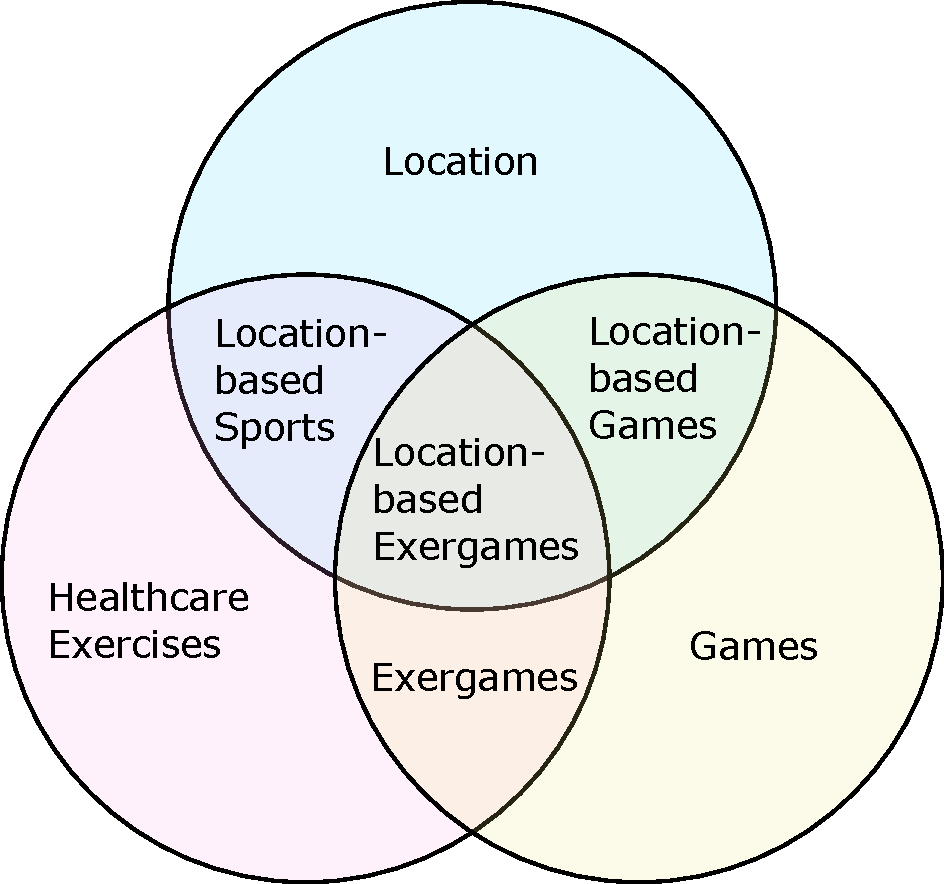
\includegraphics[width=.55\linewidth]{gfx/exergame_context}
        \caption{Context of Exergames}
        \label{fig:exergameContext}
\end{figure}

\subsection{Exergames}
A subcategory of serious games then again are exergames [41] [15]. As shown in figure \ref{fig:exergameContext}, exergames are games with healthcare exercises as added value. The term <em>exergame</em> is constructed from the words <em>exercise</em> and <em>videogame</em> [43].

The target of an exergame is to combine physical activity with fun of play. During the gameplay, the health aspect is not primarily focused but only a side-effect of playing the game. <em>“The training effect is secondary and nevertheless achieved”</em> [15]. An example for an exergame is <em>Dance Dance Revolution</em> (TODO reference). TODO: Describe Dance Dance Revolution. Bogost (TODO name) says about this game, that it produces exercise as an emergent outcome of play itself [43].

A user of the Nintendo Wii \footnote{\url{http://wii.nintendo.de/}} wrote: “Video games can [be] and are a great way to have exercise and not even know you are burning calories” \footnote{\url{http://www.gamespot.com/forums/nintendo-fan-club-1000001/wii-sports-weight-lossyesits-real-25576131/}}. Debra Lieberman found out that there is growing evidence of exergames helping people to stay fit and to manage their weight if they frequently play them [17].

So the challenge of an exergame is to keep the player motivated to do sports. As in the example at the beginning of this thesis (<em>The Running Dead</em>), we all ran away when the mob of zombies came running towards us. We did not think of doing sports in that moment. Maybe some even did not think of playing a game. Our only thought was to escape.

\subsubsection{Mobile Exergames}
Digital games are mostly completely experienced through a fixed screen. This is an obstacle to immerse into a game [38], because the player is bound to his chair and his perception is usually only stimulated by the computer screen and a sound system. In pervasive games, the interface is no longer bound to a fixed screen and to common computer periphery like a mouse and a keyboard. The player rather interacts with real world objects and real persons [39], whereas the interface of the game isn’t well defined. Any real world object could be a game object, and any real person could be a participant [14].

There is a special type of exergames, the mobile exergames, in which the player is not bound to a desktop or to a classical game board to play the game. Mobile exergames are played with a mobile device (such as a smartphone or a portable video game console). They are usually played outside and often use the location of the player to track the progress of the exercise. In most cases, the player has to move to succeed in the game, such as in Pokémon GO or StreetConqAR (which are described in more detail in chapter \ref{sec:examples}).

These games do not take place at special locations like in a gym, a laboratory or at home, separated from the real world. They are played everywhere such as on the way to school or work, at work itself, after the lunch time, after work with your kids or whenever and wherever the player (or the game, as said above for pervasive games with temporal expansion) wants to. The aim is a transformation of the player’s everyday environment into a world in play [39].


\subsection{Evolution of Location-based Games}
In the previous chapters, different types of pervasive games have been presented. Many of them depend on the current location of the player, e. g. Ingress or Pokémon GO (see section \ref{sec:examples}). This kind of games uses the current location as a basic part of the gameplay. Without the exact location, a player of Ingress could not conquer a portal and a hunter on the prowl for Pokémons would not find one nor would he find a Pokéstop to retrieve useful items. Concluded, these games would be absolutely unplayable without being able to track the location of the player with a reasonable accuracy.

Using GPS, this is only possible since May 2, 2000, when the <em>Selective Availability</em> was turned off. Selective Availability was a service to prevent civilians to perceive a better GPS accuracy than a 100 meters radius, reserving better accuracy for the military only. Since it was disabled, the GPS location is accurate to a few meters for anybody [48].

Suddenly, many location based games came up. For example, the term <em>Geocaching</em> [49] was formed during that time to describe a hunt for treasures (the <em>geocaches</em>) in the real world [50]. To find these geocaches, their locations are marked on a virtual map via GPS.

A few years later, the popular 80s game <em>Pacman</em> \footnote{\url{https://en.wikipedia.org/wiki/Pac-Man}} was transferred into a real-life version named <em>Pac-Manhattan</em> [51], using GPS sensors to track the position of the players.

With the launch of the iPhone in 2007, an era began where people always have a device at hand that is not only capable of tracking the GPS location but that is also powerful enough to run useful apps on it. This caused another hype of location-based applications.

One of it, heavily relying on GPS-based location, is Foursquare [52]. The service makes personalized recommendations of places to a user. These recommendations depend on the user’s current location and his profile. The service exists as a mobile app and as a website. Providing an iPhone app in 2009, Foursquare was one of the pioneers that combined a serious mobile application with a location-based service.

At that time, the app had a check-in feature to virtually check into specific locations. This game-like feature motivated users to visit different places to check-in and leave a Tip.

Another location-based game, that became very popular, is <em>Ingress</em> (see chapter \ref{sec:examples}). Ingress also uses the smartphones of the players to track their location and let them conquer virtual entities (named portals), that have been spread over the world.

A new member of location-based games is <em>Pokémon GO</em> (see chapter \ref{sec:examples}). Like in Ingress, players have to move in the real world, using their smartphone to discover virtual objects (like Pokémons or Pokéstops), that have been placed on real-world locations.

The real-world locations, where entities are placed in the virtual world, play an important role for these games. They have to be well-chosen to fit the purpose of the game and the respective gameplay. These special locations are called <em>anchors</em>.

\subsubsection{Anchors}
For location-based games, the real world is overlain by the virtual game world. Anchors are well defined positions, where these two worlds are blurred [26]. The word <em>anchor</em> has been introduced by Hock (TODO name) [26]. In literature, there is no fixed term for this. Other works also refer to this as <em>artifacts</em> [54] or as <em>(generic) markers</em> [53], as named in the title. This thesis uses the term anchor [26], because its semantic meaning describes very well what an anchor does: It anchors the virtual world into the real world. Another reason is, that the term \emph{marker} is already established in the context of augmented reality, which this thesis also relates to.

The placement of anchors is very important for a game and is directly associated with the user experience. Because anchors are those positions, where the gameplay usually takes place, players may easily be disappointed if an anchor is either too far away to reach it or if it is at a location not (without further ado) accessible for civilians (such as military areas, airports or the ocean). So anchors have to be placed in a way that they are accessible for all players.
Another thing is the content, that is linked to an anchor. For example, the game <em>Escape From the Tower</em> [55] lets its players reenact the escapes of some popular prisoners from the London Tower. Therefore, anchors are placed all over the tower and its surroundings with associated media. At a prison cell, this media tells the player something about the prisoner. On the staircase, the media is related to a fled, that occurred. If the content does not fit to the respective location, players will soon quit the game.

Reid (TODO name) [54] classifies the way, anchors are placed, into three categories, that will be explained in the following.

\paragraph{User-placed at Runtime}
With this method, the user places his own anchors. For this, the game has to provide some kind of editor, with which the user creates the content he needs to play the game.

The advantages of this method are, that the game can be played everywhere, because it does not depend on predefined anchors. Another advantage is, that users can create the anchors such that they fit their individual needs. In Twostone \footnote{\url{https://play.google.com/store/apps/details?id=de.tu.darmstadt.uhg}} for example, the player plays a stone-eating caterpillar that moves on a maze-like virtual track while the player moves in the real world. To win the game, the caterpillar named “Twostone” has to eat all stones, that are spread all over the track while escaping from some monsters, that try to catch it. The game includes an editor, wherewith the user can design a track by walking along the paths, where the track should be created and placing anchors at corners. The game can thus be played anywhere. Also, highly motivated and sporty players can build their own large tracks covering the whole city, whereas beginners are able to design a small one for a short sport unit during the lunch time.

Drawbacks of this method are, that a user is not a designer and may not have the required artistic skills and knowledge to produce qualitative anchors. And much less in a small amount of time [56].

Additionally, if the player desires for a quick sporting activity, he might rather go jogging in the park than starting to build a track.

\paragraph{Seamful Design}
With this method, the placement of anchors depends on features of the physical infrastructure. In <em>Feeding Yoshi</em> [54], anchors are placed on the seams of wireless access points. In the area of a secure wireless access point, the player can find a hungry creature, a "Yoshi", whereas at unsecure wireless access points, there are plantations to plant each Yoshi’s favorite fruit.

Usually, developers try to hide the limitations caused by infrastructural seams. With this method, these limitations are embedded into the gameplay [57].

Games using a seamful design to place anchors can be played at all locations, where the respective infrastructure exists. Therefore, the accessibility depends on the choice of the kind of the infrastructure. Nowadays, unsecure wireless access points are rather seldom, hence the gameplay of Feeding Yoshi suffers from this choice.

\paragraph{Designer-placed}
With this approach, all anchors are placed by the game designer. Due to the designer’s skills and insight to the respective game, the anchors are usually well-placed and harmonize with the gameplay.

As a drawback, this method is the most static and expensive one, consuming time and money until all needed anchors are placed. As a result, most games with designer placed anchors are tailored for a specific scenario, such as <em>Escape from the Tower</em> [55], which was mentioned above. The anchors in such games are often strongly related to their location. Adapting this game for another location would involve much effort.

Additional to those categories introduced by Reid (TODO name, not source), this thesis names two further categories.

\paragraph{Crowd-based Placement}
Crowd-based placement of anchors is akin to user placement, with the difference that content created by the crowd is made public for everyone. This way, the game thrives on a lively crowd of users, frequently creating new content.

Twostone, that has been mentioned before, is actually relying on crowd-based anchors, because after creating a new track, a player can opt to make the track public to be used by other players. But as mentioned in the beginning, this does only work if there is a crowd creating that content. During the release of a game, it might get challenging to build up a crowd despite the fact that there is no content yet.

Another problem is, that with a crowd, there is no control of the content. After some time, the game might contain anchors at hazardous locations such as airports or highways or it might contain pictures of morally questionable content, such as swastikas or of adult kind.

Ingress uses a crowd-based placement, combined with a designer to check the content for its propriety. Nevertheless, Ingress is only playable in highly populated areas while portals (the anchors) only exist in these regions (see Ingress map in figure \ref{fig:ingressMap}). That's because users are allowed to create anchors, indeed, by taking a photo of the desired new location, marking it on a map and sending this along with a short description to the development team of Ingress. So most requests are made for regions with a lot of citizens. But it takes several weeks, until a new portal gets accepted by the designers.

\paragraph{Automatically-placed}
This scheme describes content, that is generated automatically, obeying some creation-rules. Automatic placement of anchors helps to spread them all over the world in a fraction of time and money, a designer would need.

Actually, the seamful design is a sub-scheme of automatic placement, whereas the creation-rule is to place anchors at infrastructural seams (e. g. of wireless access points).
The rule can be well-defined, such as with a procedural content generation rule, including the use of generative grammars, spatial algorithms or pseudo-random number generators [56].
The rule can also be more complex like <em>place an anchor at each gas station marked by Google Maps</em>, which already includes some locational context.

Automatic placement also includes <em>random</em> placement. But simply placing anchors at random locations will seldomly have the result of well-placed anchors semantically fitting to their content and being accessible for everyone (e. g. oceans and deserts).

Hock (TODO name) proposed an automatic placement based on real-world objects, namely street name signs [26]. In his game <em>StreetConqAR</em>, the players have to conquer streets, identified by the name on their street name sign. Because StreetConqAR is similar to the game RacecAR GO, which is presented in this thesis, there's an extra section for this in the Examples \ref{sec:examples}.

The definition of an anchor says, that it is a "well-defined position". In the following, the term anchor is not only the position but also refers to the real-world object itself to describe the kind of blurring of reality and virtuality and the strong relationship between the anchor and its position. This blurring takes place via an object at a well defined position.

Later on, this thesis will define the term of a <em>natural anchor</em> to solve this ambiguity (see chapter \ref{sec:conceptAnchors}).

The advantage of Hock's (TODO name) approach is, that it not only saves the expanses of the a priori design of the anchors, because street name signs are already there. Also the spreading of these signs is very useful for a location-based exergame. There are very few populated regions with no street name signs.

\subsection{Augmented Reality Games}
I still remember my astonishment when I first saw the virtual shark, rising behind Marty McFly and then snapping at him in <em>Back to the Future Part II</em> (see TODO add a photo). The movie was released in 1989, wherein Marty watches the shark during his visit of the future year of 2015.

Although the year 2015 has passed, today’s technology is not able to produce such a holographic shark as it has been predicted by the movie (nor has the movie <em>Jaws 19</em> been released, the shark was advertising for).
Nevertheless, if Marty would wear some smartglasses today, he could see the shark indeed, with the help of augmented reality.

Augmented reality (AR) means augmenting perceived real-world elements with virtual media in realtime. This virtual media can be text, images, but also 3D objects or sound.

The term <em>augmented reality</em> exists for many years now. There have been moments in the past, the technology seemed likely to experience the hype, many people are waiting for. But a big hype never happened (at least until the time of writing this thesis, May 2017).

Today, there are some popular apps that use AR, such as Snapchat \footnote{\url{https://www.snapchat.com/}} (which tracks the user's face and augments it with some fancy extras like a dog's snout with matching ears and tongue) or Pokémon GO (described as one of the examples in chapter \ref{sec:examples}).

Also Apple and Facebook start to invest into this technology. Apple CEO Tim Cook even denotes augmented reality and virtual reality as potential cornerstones of the company's future. Also the coming iPhone 8 is said to be equipped with technology customized for AR [59]. Facebook CEO Mark Zuckerberg teased an upcoming games platform for AR [60]. TODO (low prio): Automotive?

Maybe, this technology is finally on the verge of experiencing a big hype.

\subsubsection{Variants}
There are different variants, all called AR. This starts with simply overlaying a video with information, that is located at specific GPS coordinates or at a tracked marker (see Technical Basics for definition of a marker TODO) and ends with exactly overlaying real-world objects with virtual objects, considering 3D position and pose.

The used variant depends on the use case and on the available hardware. The higher the grade of accuracy, with which the reality shall be augmented, the higher the requirements on the hardware, since AR is usually done in realtime. Whereas overlaying the camera picture with a virtual object while the player is located at specific GPS coordinates is a rather simple job for current hardware, tracking real-world objects from the camera picture and retrieving their position and orientation to blend the virtual object over it needs a powerful CPU that is capable of sophisticated computer vision algorithms. In the following, some common approaches of integrating virtual content into the real world are presented.

\paragraph{Square Markers}
Square markers are, as the name says, square pictures containing a binary pattern. Square markers are easy and fast to detect in a camera image and the position as well as the pose of the marker can be deduced from its binary pattern in a very efficient way. Most of the AR APIs as ARToolKit \footnote{\url{https://artoolkit.org/}} or MetaIO \footnote{\url{http://www.metaio.eu/}} provide an implementation for this kind of markers. Even current smartphones are able to track multiple square markers in realtime.

A drawback is, that the markers have to be placed in the real world beforehand. This is a disqualifier for many application fields, where the AR content has to smoothly integrate into an unprepared scene. TODO: Add picture of a hiro marker.

\paragraph{Natural Feature Tracking}
Natural Feature Tracking (NFT) refers to a technique that searches predefined features in an image. From the locations of the tracked features, the pose and location of the camera is retrieved [69]. TODO: Bild dazu, z. B. figure 2.6 von Hock.

\paragraph{Model-based Tracking}
Similar to NFT, the captured image is searched for features while these features have to match with those of a reference model. Whereas for the NFT the reference model is an image, for model-based tracking it’s a 3D CAD model. The advantage is, that with a 3D model, multiple perspectives to match the reference model to the real image are supported.
Because there’s much literature on this subject (e. g. [70]) and since this thesis’ scope only touches this kind of tracking, it won’t be described any further.

\subsubsection{Usage of AR in Games}
Nowadays, mobile devices used for AR are usually handheld devices (such as smartphones or tablets) or head-mounted displays (such as smartglasses). Head-mounted displays have an advantage over handheld devices, which are embarrassing, annoying, tedious to keep up and watch through and that are socially not accepted [58]. Additionally, a smartphone’s hardware is limited and its camera is hardly able to capture 3D structures of the real world.

On the other hand, smartphones are common and nearly everyone will always have one at hand in the near future, whereas head-mounted displays are still a rarity.

To be smoothly integrated into everyday life, pervasive games want the player to quickly immerse into the game. Augmented reality is a technology that supports the immersion effect [61], if used in the right way. Wetzel et al. (TODO name, not source) warn developers in their <em>Guidelines for Designing Augmented Reality Games</em> [62] to not only focus on a fancy technology like AR to impress the players but to rather invest in a good user experience by a lasting gameplay.

An early example for a mobile game that uses AR is <em>ARQuake</em> [63], which is an augmented reality version of the video game <em>Quake</em>. It is played outside and uses AR markers.

More recent examples are the popular games <em>Ingress</em> and <em>Pokémon GO</em>, that are described in detail in sections TODO and TODO, respectively.

Although this is a subchapter of <em>Pervasive Games</em>, not each augmented reality game is a pervasive game. A game can include augmented reality technology without expanding the magic circle.

\subsection{Examples}\label{sec:examples}
In this section, representatives of one or more of the above mentioned game types (such as location-based games, exergames and augmented reality games) are presented.

The presented games have been chosen because of their close relation to the game <em>RacecAR GO</em>, which is developed within this thesis.

TODO: Add pictures (also for StreetConqAR)

\subsubsection{Ingress}
Ingress is a location-based mobile exergame, developed for smartphones. It was developed by Niantic (TODO source) and was released in 2012. Players, called <em>agents</em>, have to decide to either belong to the fraction of the Enlightened or to the Resistance.

The anchors are designer placed and are called <em>portals</em>, which have to be “hacked” by the players to gain points for their fraction (see figure TODO image of Portal with players around).

The portals are usually located at points of social or artistic interest, such as monuments or landmarks. In contrast to StreetConqAR (see TODO), these objects are of no further relevance for the gameplay.

Ingress is no augmented reality game, although it is sometimes classified as such. It mixes reality and virtuality by the use of anchors, but is does not augment the view of the physical environment.

Ingress is considered an exergame because players have to physically move to portals to succeed in the game. The game developers, however, did not seem interested in exploiting its full potential as an exergame. Players aren’t motivated by the game to walk faster or farther. It is even possible to elude the health aspect completely by moving via car or bus to visit the portals, because the app does not check the speed of the player. It seems that Ingress became an exergame just by chance, since the developers figured out that it is entertaining to embed the virtual game world into the real world around the player [15].

Ingress is based on location data from Google Maps. Its enriched location data was used later to populate <em>Pokémon GO</em> (see section TODO) [64].

As said above, the anchors are placed by a designer. Although there exists a process for users to propose locations for new ones, which takes a few weeks to be accepted, there are many (rural) regions, where no anchors exist so far (see map in figure \ref{fig:ingressMap}). In these regions, Ingress cannot be played.

\begin{figure}[bth]
  \centering
        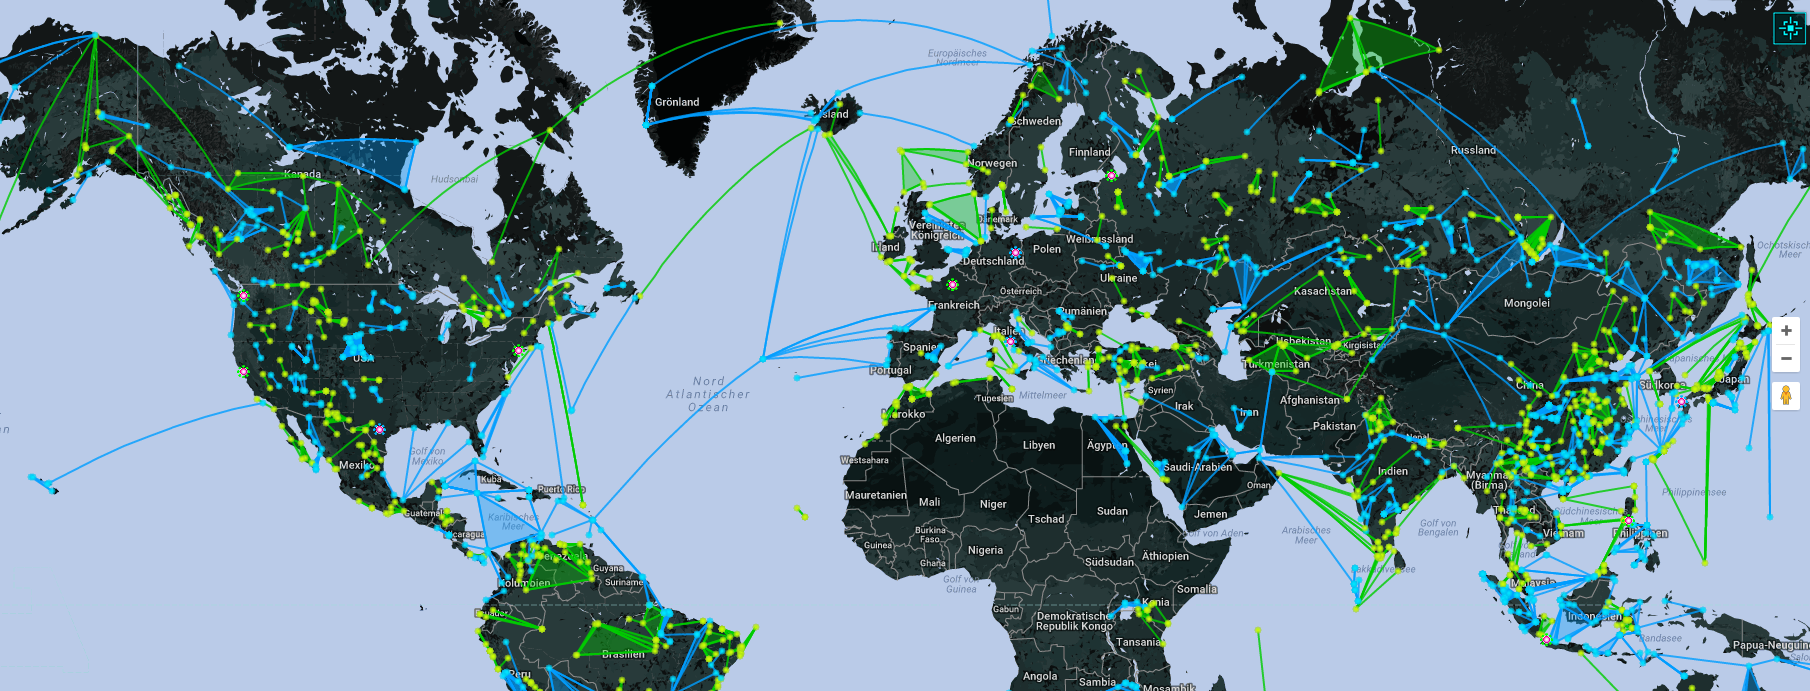
\includegraphics[width=.95\linewidth]{gfx/ingress_map}
        \caption{Screenshot of world map with Ingress portals taken with my Ingress account}
        \label{fig:ingressMap}
\end{figure}

\subsubsection{Pokémon GO}
Pokémon GO is a location-based augmented reality mobile exergame, developed for smartphones. It was developed by Niantic (TODO source) and was released in 2016. Pokémon are fantastical creatures and first appeared in the 1990s in video and card games.

A player of Pokémon GO becomes a Pokémon trainer with the task to hunt up and to catch Pokémon. Catched Pokémon are stored in the player’s Pokédex and can be trained. In Pokémon gyms, Pokémon can fight against each other. There also exist PokéStops, where some useful items can be found.

Data gathered with Ingress was used to place gyms and PokéStops [64]. These are also marked on a map that is visible when playing the game. Pokémon, however, are only visible through the smartphone display, if the player is physically near them. In this case, the Pokémon is blended above the camera video in an AR manner (see figure TODO).
To actually catch a Pokémon, the player has to throw a virtual Pokéball onto the creature. Only a well-thrown ball captures the Pokémon. Pokéballs can be retrieved from PokéStops.

In contrast to Ingress, the developers emphasize the health aspect in Pokémon GO. Though it’s still possible to visit gyms and PokéStops by car or bus, there’s a feature in the game that can only be used by walking: Brooding eggs. To brood Pokémon eggs, the player has to walk a certain distance until the Pokémon emerges. This distance can only be walked by feet since the app checks the movement speed of the player.

Another good thing is, that it does not really make sense to play this game inside. To succeed in the game, one has to go outside and walk around (e. g. to gather Pokéballs, to find new Pokémon or to brood eggs).

The virtual map that displays PokéStops and gyms also motivates the players to move. At least it motivated myself. Seeing these locations in the near environment, I though “I’m tired from work, but there are two PokéStops over there. I just visit them, maybe I find some rare Pokémon on my way”.

TODO: Add picture of Pokémon GO

\paragraph{Hazards}
Although Pokémon GO contributes to its players’ health, there are some hazards related to playing the game. There have been incidents of players walking onto rails or into restricted areas of hospitals while hunting for these little monsters [65].

There is even a website called <em>Pokémon GO Death Tracker</em> [66] that lists all deaths and injuries caused by Pokémon GO (14 deaths and 54 injuries, effective in April 2017).

\subsubsection{StreetConqAR}
StreetConqAR [26] is a location-based augmented reality mobile exergame developed as an Android app. In the game, players have to conquer streets. The player that conquered most streets wins the game. To conquer a street, one has to walk to its street name sign and watch it through the smartphone. The app recognizes the sign and displays an augmented reality version of it with virtual colored letters blended above the original letters. To acquire the street, a riddle according to these letters has to be solved.

As mentioned above, StreetConqAR presents a new way of creating anchors. Anchors are placed automatically based on real-world objects, the street name signs. The advantage of this approach is, that street name signs can be found all over the world, which means that StreetConqAR can be played all over the world, as well.

TODO: Picture

\subsubsection{Maguss}
TODO

\subsubsection{Harry Potter GO}
TODO


\section{Vehicle Recognition}

\subsection{General}
Nowadays, vision-based recognition is a hot topic. Not possible to imagine automated manufacturing without it since many years, vision-based recognition became accessible for normal users with devices like the Microsoft Kinect (TODO: reference), which is able to perform gesture recognition, for example. Another visual recognition which arrested attention (mainly because of privacy issues TODO: source) in early 2015 was Facebook’s (TODO: source) face recognition system named DeepFace \footnote{\url{https://en.wikipedia.org/w/index.php?title=DeepFace&oldid=663499386}}, which searches photos, taken by Facebook users, for people of other Facebook users.

Another field that is not so famous yet is the vehicle recognition. It is used in different systems like traffic monitoring and control or security and surveillance applications. Instead of a human observer sitting in front of some screens, an automated vehicle recognition system could do the task. Human constraints like multitasking and distinguishing among all the makes and models would be overcome by such a system.

Usually, the steps of a vehicle recognition algorithm are: (1) Feature Extraction, (2) Global Representation, and (3) Classification. Most of the systems do a preceding step and define a region of interest (RoI), which separates the vehicle from the background (see figure TODO: Either use [3]’s figure 1.4 or create a similar one in my own style - see Google Doc for State of the Art for scribble).

Feature extraction in the vehicle recognition domain denotes identifying those parts of the image that are relevant (descriptive) for this class (type, make and/or model).

The Global Representation of (Global Descriptor) can be seen as the compound of all the relevant extracted features of one image. In simple phrase, the Global Representation describes a vehicle image of a specific class such that a classifier can understand it. The key task of building a Global Representation is making it informative and discriminating. There are many different ways to construct Global Representations, some of them are illustrated below.
Finally, the classification is the process of assigning a class (type, make and/or model) to a Global Representation of an unknown class.

There are different kinds of vehicle recognition, each for a different purpose and with its own challenges.

\subsection{Vehicle Type Recognition}
For an electronic toll collection system or for the analysis of traffic jams, the actual make or model of a vehicle is not relevant. Whereas the type of a vehicle helps to deduce the properties (like shape or weight) needed for such studies. So the Vehicle Type Recognition classifies vehicles into broad categories such as sedans, SUVs, trucks, vans, motorbikes, buses, etc. [3]

As [3] mentions, most of these approaches use feature extraction and classification of different kinds. Examples are TODO.

\subsection{Vehicle Make Recognition}
Another way of classifying a vehicle is the Vehicle Make Recognition (or Vehicle Logo Recognition), which recognizes the make of a vehicle (like Mercedes, BMW, Porsche, etc.). This can either be done by solely using the vehicle’s logo or by using its whole front or back.

To classify by the logo, an image matching with logo templates can be done [19] [20]. For this, a set of vehicle logos is used as templates. Once the image snippet containing the logo has been detected, it is compared to each template using a template matching algorithm. The template with the highest match classifies the vehicle.

However, a more widely used technique is using feature detection with classification on the logo. Apostolos P. Psyllos et al. [21] (TODO name) use a database of logo images. During classification, each feature found inside the logo area of the queried image votes for each logo in the database, that contains a similar feature (evaluated by a Nearest Neighbor algorithm). The database logo with the most votes classifies the queried logo. There is one special thing about this approach, called <em>Geometric Validation</em>. It means “that the coordinates of the keypoints (features) in the query and the matched database image are checked for geometrical consistency”.

TODO: Describe approach from [22] and especially explain the bag-of-words idea (refer to chapter Technical Basics, where it is explained).

Nacer Farajzadeh and Negin S. Rezaei (TODO: name) compared these two approaches with the result, that the image matching approach performed more accurate while a feature detection method was about 80\% faster [18]. While the logo detection alone as a preprocessing step of the recognition can be very time consuming [3] and while this approach is very sensitive to occlusion due to the relatively small snippet of a vehicle image, using the whole front or back of a vehicle gives more robust classification results.

Examples for Vehicle Make Recognition are TODO.

\subsection{Vehicle Make and Model Recognition}
The most comprehensive kind of vehicle recognition and also one focus of this work is Vehicle Make and Model Recognition (VMMR), the identification of its make as well as its model (like Mercedes SL, BMW 3 Series, Porsche 911, etc.). For surveillance purposes, this recognition type extends the conventional number plate recognition. It can be used to double-check a recognized number with the corresponding make and model to fight the problem of false number plates. There are plenty of works referring to this topic and also some ready-to-use systems like Car-Rec [6] or the <em>VisualSearch</em> feature \footnote{\url{http://magazin.autoscout24.de/microsites/services/mobile/de-at/txt/android_txt3.html}} (TODO: add photo) of the AutoScout24 app \footnote{\url{https://www.autoscout24.de/}} that do VMMR.
A surveillance and security application for static cameras is eyedea \footnote{\url{http://www.eyedea.cz/make-and-model-recognition/}}, that is able to recognize 500 vehicle models of the types bus, car, truck and van.

Most of the approaches use the front or the back side of the vehicle because it’s the most descriptive part, usually containing the make’s logo and, for the back side, even the lettering of the make and the model.

While most of the systems require strictly frontal or rear view images of vehicles, Shinozuka et al. [23] proposed a solution to transform vehicle pictures taken from an angle of up to 60-degrees into pseudo frontal views.

TODO: Describe an approach based on 3D models ([2, 6, 11] from Petrovic)

The main differences among the various VMMR approaches are the construction of the Global Representations. Differences with minor importance are the choices of the local feature descriptor or the classifier, which does not mean that the local feature descriptor or the classifier have a minor effect to the classification performance, though.

<em>“The quality of a global features representation technique is assessed by its processing speed, computational complexity in forming the holistic representations, and the VMMR accuracy which reflects its discriminative capacity in representing the different makes and models while generalizing over the multiplicity issues within a make-model class.”</em> [3]

\subsubsection{VMMR using Local Features Concatenation}
One classification approach is done by \citeauthor{petrovic2004analysis} \cite{petrovic2004analysis}, achieving recognition rates of over 93\%, tested on over 1000 images containing 77 different classes (make-models). The recognition is based on a relatively simple set of features extracted from frontal car images. A feature vector of predefined length (the <em>Global Representation</em> as shown in figure TODO reference figure from above with VMMR steps) represents one make-model. The Global Representation is just a pixel-wise concatenation of the vehicle’s image. To determine the class of a queried vehicle, simple nearest neighbor classification is used among these feature vectors. The special thing about this approach is, that it uses only one vehicle image per make-model as training data. What is trained then, is the transformation of the training image into the Global Representation.

The features are not extracted from the whole vehicle image but from a RoI, a section inside of the image. This RoI is defined as an area around the car’s number plate. Thus, relative to the number plate, the RoI is independent from the vehicle’s actual location and scale inside the source image. The recognition system is shown in figure TODO (image showing (similar to Petrovic fig 2, but more detailed): input -> find number plate -> define RoI -> extract features -> Feature Vector -> Find class with nearest neighbor classification)

Starting with a straightforward representation by just concatenating the raw image values into the feature vector, Petrovic et al. ended up with square mapped gradients (TODO: definition) performing best for this purpose. TODO: Reprint [1]’s figure 5 (Feature extraction examples) as examples of different techniques with description: The structure of the original image is still recognizable (more or less clearly) because of the concatenation of image pixels
They also investigated in transforming the feature space via Principal Component Analysis (PCA) into a lower dimensional subspace to gain expressiveness and computation time. Finally though, tests including PCA performed slightly worse in most cases.

Another conclusion they made is, that a representation independent from color and contrast of the original vehicle image increases performance.

Pros of the approach of Petrovic et al. are, that the recognition process is rather easy, which means, that it includes few steps and components for both, building the classifier and recognizing a new vehicle. Thus, it’s easy to implement. It means also, that this process is easy to understand, because finding the nearest neighbor of a vehicle image in any kind of representation-space seems plausible to work properly.

There are also cons of their approach that will occur, when testing the system in real-life conditions. While the vehicle’s Global Representation (its feature vector) is based on all of the pixels contained in its RoI, the recognition will not be robust to occlusion of some part of this area. For the same reason, slight changes in the camera’s roll-angle or a displaced (or badly captured) number plate will also decrease the recognition performance. Hence, such an approach is not applicable in real-life scenarios.

\subsubsection{VMMR using a Bag-of-Words Model}
Another approach that tries to eliminate all the cons of the system proposed by \citeauthor{petrovic2004analysis} is made by A. J. Siddiqui [3] (TODO name). Since that system is similar to the system proposed in this thesis, it will be discussed in more detail, here.

The challenges, [3] attends to, are <em>multiplicity</em> and <em>inter-make and intra-make ambiguity</em>. <em>Multiplicity</em> describes the problem of vehicles with different shapes or appearances all share the same name (make and model). An example for this is shown in figure TODO reprint [3] figure 1.5 “reprinted from [3]”.

While <em>inter-make ambiguity</em> describes the issue of models from different companies being akin to each other, <em>intra-make ambiguity</em> refers to different models from the same company that share similar features. Examples for this are shown in figures (TODO reprint [3] figures 1.6 and 1.7 “reprinted from [3]” Inside State of the Art, reprint figures of vehicles from sources, because I talk about it in their context. Inside Concept chapter, I use MY vehicle images)

So the task is to build a Global Representation, “that accounts for intra-class differences and inter-class similarities, thereby solving the multiplicity and ambiguity issues in VMMR” [3] and that is robust to occlusions and small changes in the camera angle.

In contrast to the approach of Petrovic et al., the Global Representations of this system are constructed using a bag-of-words model (TODO: See chapter Technical Basics for explanation) instead of concatenating the pixel values of the RoI. This means, similar to the Vehicle Make Recognition system proposed by [22], mentioned above, the Global Representation is a histogram. Each bin of this histogram represents one distinct feature-codeword while the height of the bin indicates the occurrence-frequency of this specific feature-codeword in the source image.

The set of all feature-codewords, the <em>visual words</em>, build the dictionary or <em>bag</em>. A feature-codeword in this context is not a feature but a representative of several similar features. This way, the size of the dictionary does not only control the size of the Global Representation (number of bins in the histogram) but also the threshold, at which several features are clustered into one single dictionary feature-codeword. So the dictionary represents the essence of the key features (in this case SURF [31]) of all the training images.

\paragraph{Dictionary Generation}
Two different schemes of dictionary generation are proposed. One called <em>Single Dictionary</em>, the other called <em>Modular Dictionary</em>. For the Single Dictionary, all the local features of all training images are clustered. Each cluster center then represents one codeword of the Single Dictionary. The number of clusters defines the size of the dictionary, therefore. An advantage of this scheme is, that considering the combined set of features over all the training images (across multiplicity and ambiguity) strengthens the discriminability of this dictionary. A disadvantage is, though, that one cluster could contain features that are similar but originate from different make-model classes. To cope with this, a dictionary is only built out of the training images for one specific make-model class (in the same way as described above), resulting in one dictionary per make-model class. The set of all the codewords of those dictionaries form the Modular Dictionary. An advantage, besides the one noted above, is the flexibility when adding new training data. Only the dictionary of the specific class has to be rebuilt, which saves processing time. A disadvantage is the increased size of the Modular Dictionary compared to the Single Dictionary. Although the size of one of its per-class dictionaries can be smaller than that of the Single Dictionary, multiplying this with the number of make-model classes will boost the number of overall codewords. For an illustration of the two schemes, see figure TODO: reprint figure 3.15 from [3] and explain the variables in the footer.

\paragraph{Results}
For the classification (step 3 of vehicle recognition process TODO: Reference image from above), a multi-class SVM (TODO reference SVM in Technical Basics)-based classifier is used. The classifier is trained to learn both similarities among different generations of the same make-model class and differences among inter-class models.

Experiments showed that the Single Dictionary, contrary to the expectations, slightly outperforms the Modular Dictionary. On the other hand, the dictionary training time is much less for the Modular Dictionary. However, for an application, where the dictionary is built offline and does not need to be updated (or only seldomly) during runtime, the Single Dictionary is the better choice.

Additionally, the bag-of-words model implicates some advantages in contrast to the local features concatenation approach by \citeauthor{petrovic2004analysis}. Because the Global Representation is not directly depending on the pixels-grid of the source image, it is robust to occlusion to some extent. As long as the remaining set of local features is descriptive enough, the vehicle can still be classified (see figure TODO show classification of test image with occlusion). Another advantage is the robustness to slight changes in the camera roll-angle or in the perspective. Due to the local descriptors, in this case SURF, that is rotation invariant, rotated local features would still result in the same bag-of-words histogram.

A downside of this approach is, though, that the local features lose their spatial information on their way into the Global Representation. The original position of a local feature is neither encoded inside of the local feature descriptor nor inside of the global descriptor. So an image with same features which are in a different order gets the same match. TODO: Show two images, one of the front of a vehicle, another, the same image but with parts of them disordered and maybe multiple times occurring. Then show the histograms for both of these images (→ same histograms).

To solve this problem, a <em>Geometric Validation</em> as seen in the Vehicle Make recognition system proposed by TODO [21] could be applied. Another way to retain the spatial information of a local feature to some extent is to use a grid-based Global Representation (TODO: describe how this would look like, look at [3] 3.2.1, and see scribble in State of the Art Google Doc)
TODO: IMPORTANT: A proposal to solve this should NOT be made inside State of the Art!!! And only do this, if there's enough time at the end.


\section{Number Plate Region Detection}

\subsection{Definition}
In contrast to “Number Plate Detection” or automatic license plate recognition (ALPR), where (also) the content of the number plate is desired.

TODO: Reference already working Systems. I heard that automatic recognition is used in Österreich to recognize the Vignette.

TODO: Refer to [7] and [8], [9], [10]

TODO: Explain Hough Transform in detail with image and formula and such (as Hock did in Technical Basics)







%*****************************************************************************
%*****************************************************************************
\chapter{Concept}\label{ch:concept}
%*****************************************************************************
%*****************************************************************************
This chapter is about a new way of automatic content generation for exergames. It presents an approach to use real-world vehicles as anchors. Using vehicles as anchors means recognizing their make and model and integrating its virtual counterpart via AR into the game play.

In the first section, the basic concepts needed for a location-based exergame and what makes such a game popular are discussed. Later on, the design of <em>RacecAR GO</em>, a location-based exergame that implements this concept, is presented. In the subsequent section, the prototype of RacecAR GO, that will be implemented along with this thesis, is described.

As VMMR is an important part of this game, an approach for this is proposed in the final section of this chapter.


\section{Location-based Exergame using AR}
This section is about the preparation and evaluation of the basic concepts to build a location-based exergame. It first discusses the type and how to integrate anchors, then it generally evaluates the properties of such games that motivate people to play and to move. Later, the usage of augmented reality as a technology to improve the user experience is discussed. A list of requests for a location-based exergame as a result of this evaluation is presented in the final section.

\subsection{Anchors}\label{sec:conceptAnchors}
As a reminder, <em>“anchors in pervasive [...] games are well defined positions, where reality and virtuality are blurred”</em> [26]. An exergame that shall be playable all over the world also requires anchors placed all over the world.

In the State of the Art chapter (see TODO), many approaches for creating anchors have been proposed with pros and cons. It turned out that designer placed anchors are usually well-placed and well-fitted to the game’s purpose, but include an expensive design process. As a result, games with designer placed anchors mostly provide content for only a few limited regions.

On the other hand, placement of anchors by the users takes the work out of the designer’s hands and provides the possibility to create content all over the world. As a drawback, the quality of such anchors usually suffers and depends on the goodness of the editor and on the user’s design-skills. Another disadvantage is, that the user must pass the design-phase before he is able to play the game. Such an approach is not suited for a game that smoothly integrates into the player’s everyday life and shall every time be playable without any pre-setup.

The automatic anchor generation offers a good middle course for this request, as it doesn’t include an expensive design process but nevertheless produces well-placed anchors depending on the creation rule.

\subsubsection{Natural Anchors}
\citeauthor{hock2014augmented} proved in his thesis, that placing anchors at street name signs creates a game that provides content for many regions (urban and rural ones) all over the world \cite{hock2014augmented}. Additionally, he not only used the positions of the street name signs but also included the object itself as an anchor into the game. This comes with some ambiguity issues, because the term anchor is used for both, the location and the related object.

As a solution, this thesis introduces a new term, the <em>natural anchor</em>, which is an object, that exists in both, the real world and the game world. At its position, the reality intersects with the virtuality.

This means, that the real object and the virtual object are semantically the same. In Hock’s (TODO name) game <em>StreetConqAR</em>, a street name sign in reality is also a street name sign in the virtual game world. In contrast to that, anchors in Ingress or Pokémon GO are often placed at distinct objects like monuments or landmarks, though, but in the game world, the semantic meaning of these objects is different. They turn into portals for Ingress and into PokéStops or gyms for Pokémon GO.

This thesis proposes to use real-world vehicles as natural anchors for an exergame. The way these are integrated into the gameplay and a discussion about the characteristics of this special type of anchor can be found in chapter TODO RacecAR GO and TODO RacecAR GO->Anchors, respectively.

\subsection{The Art of Motivating People to do Something for their Health}
In the previous chapter, many different examples of exergames have been listed, each having its own approach to motivate its players to do something positive for their health. The key seems to be to encourage the players by something that is fun. This something’s main intention is not doing sports. The health aspect is just a side-effect of playing the game.

In the following, the concepts used by various exergames to motivate their players to move are compared and discussed.

An often used motivation is to achieve (virtual) property. It seems that players keep on playing a game as long as there are achievements of some kind to accumulate their (virtual) property. This concept is used by Pokémon GO, for example, where the property is the personal Pokédex with the captured Pokémon. It is also used by Ingress where the property are the hacked portals. Additionally, the player could form an emotional relation to its property, which also keeps him on playing.

Another concept, akin to achieving property, is the achievement of reputation. The more and the harder a player trains, the more reputation he can get inside the game. This is used in StreetConqAR by giving the players titles as "King of ..." or "Lord of ...", in Ingress by gaining experience points or in Pokémon GO by becoming a Pokémon master.

In the exergame <em>The Running Dead</em>, proposed in the beginning of this thesis, a simple but strong motivation to run is used: Fear. Fear of what will happen if a zombie catches me.

A motivation that is deeply anchored into the human’s roots is based on the hunter-gatherer principle.

\subsubsection{Hunter-Gatherer Principle}
Long time ago, when our civilization was young, most of the people were hunter-gatherers. This means, people spent a big part of their lives with hunting for animals or gathering fruits to eat or items to construct tools of. For such a civilization, these things were necessary to survive. After some time, people became farmers and the number of hunter-gatherers decreased.

Today, most people aren’t hunter-gatherers (nor are they farmers). But although our everyday life differentiates so much from that of a hunter-gatherer, a desire for this kind of life still seems to be lurking in many of us. Why else would there be millions of people playing Pokémon GO, in which the main task is to hunt and to gather little monsters?

\subsection{Augmented Reality}
As discussed in the State of the Art chapter, augmented reality is an up-and-coming technology used in many application fields. Utilized in a pervasive game, it can help the player to immerse into the game. But using AR as a fancy technology for its own sake isn’t the right way to design a good game. It’s better to focus on a lasting and catching gameplay and using AR to support this instead of trying to impress the player with stunning technology [62].

\subsection{Requirements}
To create a successful exergame that motivates its players to do something for their health, following requirements (\emph{GR} for game request) can be deduced from the previously said:
\begin{description}
  \item[GR1:] The game has to be playable everywhere at anytime
  \item[GR2:] The players must be able to start a game session without needing any previous setup
  \item[GR3:] The game uses a principle to motivate players to move
  \item[GR4:] The game integrates augmented reality in a reasonable and supporting manner
\end{description}
\emph{GR1} contains two aspects of the game. The first one relates to the game’s platform and the needed hardware. To be playable everywhere, the game should run on a mobile device. The second aspect is the game content (the anchors), that has to be available everywhere a player could have the idea to go for a quick session.


\section{Concept of RacecAR GO}
TODO: Icon of RacecAR GO goes here (small with much margin, about half a page)

In this section, the concept of the game <em>RacecAR GO</em>, that uses real-world vehicles as anchors, is presented. It shows approaches to fulfill the previously declared \emph{GRs} and also discusses challenges that accompany them.

\subsection{Overview}
RacecAR GO is a location-based exergame. It’s played outside on a mobile device. The player’s task is to find and capture vehicles by taking a photo of them with the device’s camera. The virtual counterpart of each captured vehicle is then stored in the player’s virtual garage. At certain locations, players can compete against each other to win other player’s cars or to lose the own ones.

Not only is the name RacecAR GO akin to Pokémon GO, also the gameplay is. This is because Pokémon GO motivated millions of people to play and to move, so its concept can be regarded as exemplary.

\subsection{Platform}
RacecAR GO is realized as a client-server app. The client app is available for both, iOS and Android. The advantage of current devices running iOS or Android is, that they usually come with a GPS sensor and mobile internet. The server stores and manages all user data and attends to the recognition of the make and the model of a captured car (for an illustration with some exemplary tasks see fig. (TODO: Picture that shows the communication and the tasks of each side.
Client: camera capture of vehicle, AR, location-tracking
Server: VMMR, User-Management, Game-Data handling)
See scribble in google doc
)

\subsection{Story}
TODO:
Hier das Storyboard zeigen. Die einzelnen Bereiche werden in den folgenden Sections erklärt, wie z. B. der Capturing-Process. Dort wird dann wieder auf das Storyboard hier verwiesen.
Storyboard:
Anzeige von Wert eines Autos
Anzeige des gesammelten Geldes

\subsection{Gameplay}
The gameplay is described on the basis of the storyboard (see section TODO). Each subsection inside this section refers to one of the storyboard’s views. A player starts the game by creating an account or by being automatically logged in with his existing account.
The game has a centralized structure, i. e. each view is accessed via the menu. With a <em>Back</em> button, the user can always return view by view back to the menu. The menu has six entries, each representing one area of the app:
\begin{description}
  \item[Capturing:] To capture new vehicles
  \item[Garage:] Shows all captured vehicles with its properties. Vehicles can also be upgraded here
  \item[Map:] Shows a map displaying nearby car dealers or playgrounds
  \item[Car Dealer:] To sell captured cars to
  \item[Playground:] To compete with other players
  \item[Settings:] Shows the game settings
\end{description}
The user is able to achieve money during play, so his current credit is always displayed at the top bar of the game. This is for a motivational reason, because the player earns money by physically moving with a speed less than seven km/h. So always displaying the current credit will motivate him to walk farther and watch it increasing.

\subsubsection{Capturing}
At the start of the game, the player finds himself directly in the <em>Capturing</em> view, ready to capture new vehicles for his garage. This fulfills GR2 which demands that the player must be able to play without any annoying setup. This view is also accessible via the menu. The capturing process is divided into four steps and is illustrated in figure TODO.
\begin{enumerate}
  \item As long as the capturing process is in step 1, the device shows the vehicle as the camera takes it. To capture it, the player has to point the device's camera towards the desired vehicle's front view or back view. In the background, the app sends a picture of the vehicle to the server. The picture has to be the front view or the back view, because along with the picture, the hashed number plate is sent to the server. This is to check, if the user hasn't captured the car yet. If he has, he cannot capture it for a second time.

Otherwise, the server performs a VMMR (see section TODO) and sends the retrieved make and model along with its respective properties (in the example a "VW K\"afer" with a matching property-set) back to the client.
  \item With the received make and model, the app chooses the correct virtual vehicle with that make and model and blends it above the real vehicle (see section TODO Augmented Reality in this RacecAR GO section for details).
The player is then able to walk around the real vehicle while he only sees the virtual one through the device. He can interact with the vehicle by touching on the door or on the hood to open and close it. To continue, the player has two options. He can either touch the trash icon and abort the capturing, or he can opt for the garage icon, to park the vehicle in his garage.
  \item To park the vehicle in his garage, the player first has to fulfill a small task. For the task, a vehicle part appears that matches to the captured vehicle. This part could be a door, a steering wheel, a car seat, an engine or another part the captured vehicle consists of. In the example, it’s an engine. This part overlaps the vehicle and is fixed to the device’s screen, such that when the player moves around the vehicle, the part overlaps different areas of it. The player's task is to place this part at the correct position. E. g. for the engine and the VW K\"afer (which has a rear engine), the user would have to walk around the car, touch on the engine cover to open it, place the engine at the correct position (by moving the device such that the engine icon overlaps the position where the engine of the real car would be) and finally touch the wrench icon.
  \item If the placement is correct, the vehicle will be parked in the player's garage. If not, the capturing will be aborted. The vehicle is stored along with its property-set, containing its power, weight, emission, etc. This data is retrieved from an API like <em>CarQuery</em> \footnote{\url{http://www.carqueryapi.com/}}. In most cases, it's ambiguous to deduce the property-set from a vehicle picture, as the appearance of the vehicle doesn’t change (or only marginally) for different engine configurations. For this reason, the server would have to search clues in the picture, like the exhaust or additional letters on the backside or the grill of the car that indicate a distinct configuration.
\end{enumerate}

TODO: Also retrieve the vehicle’s color by extracting it from the picture and matching it with available colors from the manufacturer for that model

\subsubsection{Garage}
The captured vehicle is then parked in the player’s garage. The garage can only be accessed via the menu. It lists all the vehicles, the player has already captured. Touching one vehicle item opens the vehicle’s details. Inside the details, the vehicle’s properties as well as its 3D-model are shown. If there’s a small arrow behind a property, it means that the player has enough money to afford an upgrade for that property. Touching the arrow performs the upgrade and pays the money from the user's credit.

\subsubsection{Map}
The map shows the surroundings of the player. Its purpose is to visualize the location of nearby car dealers and playgrounds. Locations of car dealers are marked with a vehicle symbol, playgrounds are marked with playing cards. The player is always in the center of the map.

\subsubsection{Car Dealer}
This view is, like the playground, only available, if the player is physically near to a car dealer marked in the map. Here, he can sell his captured cars. This might be useful for frequent cars, as the player should usually have plenty of them in his garage. Nonetheless, the dealer pays a much better price for rare cars.

\subsubsection{Playground}
TODO: Here, describe the process of playing happy families. Also refer to upgrades , because only now the reader understands, why a car can get upgrades.

TODO: Show picture of a happy families play card.
The design of the play card in my game should look like one of these, at least in the design in this thesis.
Properties:
Eco bilance
See Notes

\subsubsection{Settings}
In the settings, the player is able to change his password and to enter the battery saving mode (as in Pokémon GO) which turns off the screen if it is not directed towards the user. This is necessary because an app with these requirements will consume much battery power. The durability of the battery would otherwise be a killjoy for motivating the player to move and to immerse into the game.

\subsection{Usage of Anchors}
This section is about the types of anchors that are used by RacecAR GO and about their implications. As described in the gameplay section TODO, the game content includes three different location-based items that serve as an anchor: Vehicles, car dealers and playgrounds (actually there are four, as the user can be regarded as a natural anchor itself, since he is integrated into the game as himself, at least in the map view).

In the following, the choice of the anchor for each of these items is discussed.

\paragraph{Vehicle Anchors}
In the game, vehicles function as natural anchors. This means objects, that exist in both, the real world and the virtual world. The big advantage of such anchors is, that they do not have to be distributed a priori by a designer, they are already there.

A special characteristic of the vehicle as anchor is, that it tends to be not fixed in its location. This breaks the criterion of an anchor as a “well-defined position” [26]. But since the vehicle as natural anchor does only persist during the capturing process, where its location is fixed (hopefully, but see section TODO for hazards), this fact hasn’t any impact on the gameplay.

A positive effect of using vehicles is, that urban areas become attractive to walk in. As Gehl (TODO name) states, today’s cities are car-friendly and unwalkable [68]. People usually don’t find it very attractive to do sports there, like jogging or cycling. From the perspective of this game, these are good prerequisites to play at. Being on the prowl for seldom vehicles, a car-friendly and unwalkable environment turns into a paradise.

In contrast to the anchors placed in Ingress or Pokémon GO, the actual distribution of the vehicle anchors cannot be controlled by the game. The distribution changed continuously and cannot be tracked as a whole. For the capturing process, only the local distribution is important. Considering the map showing the number of vehicles per capita for regions in the whole world (see figure TODO World-vehicles-per-capita from drive images and reference "reprinted from" [67]), there are only a few regions, where it could be difficult for a player to find enough vehicles to have fun playing this game (e. g. in Central Africa or in parts of Asia). So the predefined \emph{GR1}, that the game has to be playable everywhere at anytime, is fulfilled by the vehicle anchors.

There are also some drawbacks, though. The real-world part of the natural anchor does not have to be distributed, indeed, but the virtual part, the counterpart of each real-world vehicle, has to be created a priori. The VMMR machine has to be trained for each make-model as well. A solution to this problem is to only cover a limited amount of make-models. These include the most-frequent ones, like the VW Golf, which exists nearly all over the world, but also a few rare models. With such a starter-set, the game can be played everywhere, whereas only a subset of the cars around the player can be captured. A crowd-based approach to extend this starter-set is possible. If a player tries to capture a vehicle, that is not yet supported by the app, he would be asked to specify the make and the model. The VMMR machine could then use this data to train itself. The missing virtual vehicle counterparts could also be submitted by a crowd. As it is done for Ingress, there should be a reviewer to check the user-created content.

TODO (low prio):
With every recognized vehicle, the classifier improves itself (for this, there are special players, who must rate the done classification as right or wrong)
TODO: Show a small workflow for this (get pic -> classify -> ask user if correct -> improve classifier).
Works for all kinds of vehicles, like cars, trucks, motorbikes, buses

\paragraph{Car Dealer Anchors}
Car dealers are also represented by natural anchors. This means, that car dealers in the game are also car dealers in the real-world. The location of car dealers can be retrieved from Google Maps. The advantage of using this type of anchor is the semantically sensible inclusion of car dealers into the game. It's safe to assume that the distribution of car dealers in the world is well-suited to the game's needs. Where there are cars, there have to be car dealers. If there's a region that lacks car dealers, the game can still be played, as selling captured cars is not essential for the gameplay.

\paragraph{Playground Anchors}
As opposed to this, playgrounds are an essential part of the gameplay, without which all the hunting and gathering would be aimless. For this reason, well-distributed anchors are needed. Whereas most vehicles need gas to drive, gas stations can be considered as well enough distributed, such that most players are able to visit one without much effort.

\subsection{Usability}
TODO (low prio):
Easy to use, no (complicated) setup, start immediately
Designing the UI of MaM - user focussed, referring to Oppermann 1.3.3.1, 1.3.4.1, participatory design - not only UI but the design of the whole app (software, technology, UI, …)
Discuss devices to use: Handheld (smartphone, tablet), head-mounted - see Hock 3.3.1
Prerequisites to play: Smartphone (limitation to iOS later) with mobile internet access, a camera (and GPS?)

\subsection{Users}
TODO (low prio):
Accounts on server
How to get account? TODO
User can login with his credentials from arbitrary device to play.
Also login via browser without geo- and camera-dependent actions like capturing cars

\subsection{Usage of Augmented Reality}
As denoted in the gameplay, augmented reality is used inside this app to blend the virtual vehicle above the real vehicle during the capturing process. It is expected that the way of blending the real and the virtual world - by the transformation of a real car over an augmented car into a virtual car - greatly improves the immersion effect for the player (\emph{GR4}).

The task is to blend the virtual vehicle in a way above the real vehicle, such that both objects overlap perfectly and the player is able to walk around the vehicle to regard it from different views. To solve this task, there are multiple approaches, which are discussed in the following.

\paragraph{Square Markers}
As described in State of the Art (TODO reference), square markers are very efficient to track, even for mobile devices. Using square markers for the vehicle capturing process would implicate that there have to be square marker pictures being placed on the real-world vehicle, which isn’t the case.

\paragraph{Number Plate as Marker}
This approach uses the vehicle’s number plate as the AR marker. The marker tracking is realized with NFT (see TODO State of the Art -> Natural Feature Tracking). During the capturing process, the number plate of the vehicle gets detected. When the camera moves, the tracked features from the number plate are used to calculate the location and pose of the vehicle.

ARToolKit (TODO reference) provides an implementation for this for mobile devices. The realtime-calculation of the location and pose of the vehicle from its number plate performed quite well, producing robust results for blending the virtual vehicle above the real one (although this only works for perspectives, where the number plate is visible, i. e. not for the vehicle’s side view). But the initial tracking of the number plate’s features took up to a minute (for a number plate width of 100px on a Intel i7 of the year 2012). This is because the process has been designed to train the feature recognizer in an offline phase and just use it in the online phase without changing the set of known features. Since the number plate of the captured car is not known in the offline phase and since the player doesn’t want to wait one minute until the AR magic begins, this technique is not applicable.

\paragraph{EURO-Badge as Marker}
In most european countries, a number plate contains a euro badge (see TODO image). In contrast to the number plate, features of the euro badge can be tracked in the offline phase, because the badge is the same on each number plate.
Tests with ARToolKit on a mobile device resulted in an improper calculation of the location and pose of the badge, which was perhaps down to the fact that there aren’t enough (unambiguous) features to track inside this badge image.

\paragraph{Model-based Tracking}
As described in State of the Art (TODO reference), this approach relies on a 3D CAD model as reference to identify features in the captured image. Based on the reference model, its pose inside the captured image can be deduced from any perspective. Since the 3D CAD models are already present (the virtual vehicle models), this approach is very suitable to fulfill the requested task.

\paragraph{Smartphone Motion Sensors}
Another option to blend the virtual vehicle appropriately above the real one is to use the mobile device’s motion sensors. In contrast to the aforementioned methods, this one is not vision-based. To initially fix the virtual vehicle to the real one, the position of the number plate is used. From that time on, the motion of the device is appropriately applied to the virtual object such that the player can move and rotate the device while the virtual object is fixed above the real vehicle.

This approach works well in tests, although the virtual object and the real object drift apart over time. This is because the virtual object is only once (in the beginning) stitched to the real vehicle. After that, accumulating errors in the device motion updates could account for the drift.

\subsubsection{Conclusion}
Only the model-based tracking is able to fulfill all the requested tasks accurate enough. Only here, the user would be able to walk around the real car while the virtual car model is always overlaying it correctly. Nevertheless, it is assumed that this technique has high hardware requirements, because features in the camera image have to be tracked and matched with the reference model in realtime.

\subsection{Privacy Concerns}
TODO:
Photographing property of other people
Photographing number plate and sending it to the server
Hashed for capturing
unhashed as marker for AR
Not storing any photographed data
→ Use a disclaimer and instruct players to behave adequately when playing is enough?

\subsection{Hazards}
As proved by Pokémon GO, the hazards accompanying a game that is played outside are not of a minor kind. There have even been cases of death, according to the <em>Pokémon GO Death Tracker</em> [66].
TODO:
Discuss hazards (city traffic), unwanted public disturbance, unwanted locations (car dealer, private property?), attention at worst possible times or too much attention in general

Running onto the street to take a photo of a driving car (maybe if the marque is very seldom)
Gas stations as playgrounds: At gas stations, there is usually a lot of traffic. Crowds of people standing there and playing RacecAR GO could for one thing cause a jam and for another thing endanger themselves when carelessly standing in the way of driving cars.

Compare to hazards (and really occurred cases) of Pokémon GO

\subsection{Fake Check}
TODO (low prio):
How to realize such a Check?
Is it necessary? Evaluate this. Guys who want to play do usually not want to fake
One is to store the number plate to hinder player to capture same vehicle multiple times (see TODO link Vehicle Recognition and Capturing Process)
Capturing the photo of a car also works. How to prevent this?
Check that players move by feet and not by car while playing the game: Like Pokémon GO (brooding eggs), the player has to be rewarded for walking by feet. For a walked distance, he could earn money to tune his cars. Although there is no deeper relation between walking by feet and earning money. Fake check would then be to only earn money for movement with speeds less than seven km/h. ( ← only the speed check belongs to this section. The earn-money-thing belongs to another section).

\subsection{Business Model}
TODO (low prio):
Scalability
Like Ingress and Pokemon GO: Companies pay for their locations to be used as anchors in the game, Such that players visit their company to succeed in the game
Vehicle Trading Companies pay money to get their makes into the game or to get an area inside their trading houses where virtual cars can be bought for real money

\subsection{Classification as a Location-based Exergame}
In the previous chapter, exergames have been defined as video games, that combine healthcare exercises with gameplay fun, whereas the healthcare aspect is not primarily focused. To succeed in the game, however, physical activity is necessary.

RacecAR GO fulfills these criteria. To succeed in the game, players have to physically move to vehicles, car dealers or playgrounds, which are location-based. The primary focus of the gameplay is the hunting and gathering, though. This is also the motivational principle (\emph{GR3}), that is used by the game. Another principle to motivate the players to move is the achievement of (virtual) money when walking by feet.

The game also covers concepts of pervasive games, such as breaking the magic circle in a spatial and temporal manner. As a result, it integrates smoothly into the player's everyday life: Players would be encouraged to walk through their environment with eyes open to discover a vehicle that is desired for the game.

\subsection{Comparison with other Exergames}
TODO (low prio):
Constraint when playing at night: Can only be played when there’s enough light to get good VMMR results (Ingress and Pokémon GO independent of light)

Setting must be urban, so that there are cars near to the player (Ingress and Pokémon GO can also be played in rural areas, or generally everywhere, AS LONG AS there are (artificial) anchors placed)


\section{Concept for a RacecAR GO Prototype}
Along with this thesis, RacecAR GO will be implemented prototypically. To match the timeframe of a master thesis, a reasonable subset of features will be defined in the following.

\subsection{Limited Story}
TODO: Here, print the storyboard with all the views, that are included in the prototype.

The prototype focuses on the hunting and gathering of vehicles. The upgrading and selling of vehicles as well as the playground has been omitted. Without these features, a map would be useless, so it has been omitted, too.

\subsection{Platform}
The prototype will only be implemented for iOS, especially for iPhones. The implementation excludes the iPad, because the game requires a mobile device, that the player always carries with him and that is compact enough to walk through the city with. It’s possible to play RacecAR GO on the iPad, however, but to experience a smooth integration of the game into the everyday life, the iPhone is the better choice.

\subsection{Users}
TODO (low prio):
No user-management on the server-side. User-data is holistically stored on the client (name, gathered vehicles).

\subsection{Vehicles}
The type of vehicles that shall be capturable in RacecAR GO can be of an arbitrary kind, from motorbikes over racecars to trucks. A limitation for the prototype is, that only passenger cars are covered by the app. This is due to the fact, that the VMMR machine, that will be implemented along with this thesis, recognizes vehicles solely based on their front. More precisely, a specific region around the vehicle's number plate is chosen to classify the vehicle with. As motorbikes don't have a wide front and in most cases don't even have a number plate, they are not covered by the prototype. The problem with trucks (or buses) is, that the region around the number plate of a truck is not descriptive enough to differentiate it from other trucks of a different make and model (for further reading see the drawbacks in chapter \ref{sec:regionAroundNumberPlate} or refer to the ambiguity issues in TODO: State of the art: VMMR using a Bag-of-Words Model).

As described above, the app comes with a starter-set of vehicles, that can be recognized and captured. For the prototype, this set is limited to 10 TODO different vehicles. See (TODO respective impl chapter) to see, which make-models have been chosen and why. Unlike to the full version of the app, there is no possibility to add further make-models but for the game designer to add them manually.

For each covered make-model, there is only one property-set, that is automatically applied to the respective captured vehicle.

\subsection{Vehicle Capturing}
There are also some restrictions that have to be done for the capturing process.

TODO: Show the part of the capturing-storyboard that has changed for Limited: Capturing of vehicle with number plate watermark!!

Show picture of shortened capturing-workflow with additional steps:
Because the vehicle will be recognized based on a region around its front number plate, first capture the number plate (with water mark)
Extrakt roi
Send
Classify (ignore number plate, a vehicle can be captured multiple times)
Receive make, model (without property-set)
Select matching virtual vehicle model
… blend over, fix at number plate, use device sensors
No interaction
Virtual Vehicle models are stored client-side. This is possible for a few models. For more, another solution is necessary
No mini-game, vehicle is directly stored in garage

\subsection{Augmented Reality}
Because the recognition of the vehicle is fixed to its front and since the capturing task with fitting the vehicle parts will not be implemented, it’s sufficient to overlay the real vehicle with the virtual one in the front view.

For this, three of the aforementioned approaches come into question. First one would be to use the vehicle’s number plate as AR marker. As mentioned above, the test results of tracking the marker and calculating its pose and location were quite well whereas the initial setup of this marker took too long for a reasonable user experience.

Another approach is the model-based tracking, which was proposed to be used for the full version of the app, because it is able to calculate the vehicle’s pose and location from arbitrary perspectives.

The last approach is to use the smartphone’s motion sensors to deduce the vehicle’s pose and location.

Both, the second and the third approach are applicable to the task. Because of the expectedly high computational resources needed for the model-based tracking on a mobile device, the third one will be implemented.


\section{Concept of Vehicle Make and Model Recognition}
In this chapter, the VMMR system that is used in <em>RacecAR GO</em> will be presented. Until now, the work on vehicle recognition has mainly been dedicated to the subject of security observation of parking spaces, toll stops, country borders, etc. In this thesis, the domain of application is something different, using it in a mobile game and capturing the vehicle images with a mobile phone's camera.
TODO one more sentence to lead to Ambiguity and Multiplicity section.

\subsection{Excursion to the Ambiguity and Multiplicity Challenge}
As stated by [3], the assembled recognition model should cope with ambiguity and multiplicity issues. Multiplicity means the problem of cars with different appearances but with the same make and model, whereas the ambiguity describes the challenge to differentiate between similar vehicles that do not have the same make (inter-class ambiguity) and/or model (intra-class ambiguity), though.

Assuming a player of RacecAR GO walks along the street and suddenly, he spots a Porsche 911 parked beside him. Fortunately, in front of the Porsche, there's enough clearance to take a photo of its front. Already imagining himself watching this beautiful and seldom car in his virtual garage, wouldn't it be annoying if the app would classify this Porsche 911 as a rather ordinary Mini One, just because of the similarity between the shape of their headlights (see figure TODO: Picture with both cars. Mark both features in the image and also show two histograms, where the same bin would increase because the same codeword would be found. Describe this part of the image later, when the histogram is explained)? Such a failure could kill all the motivation of a player to continue playing, and thus losing the healthy benefits of this game. As a result, the game would miss its purpose to motivate people to move.

Due to the small number of realized makes and models for the RacecAR GO prototype, these can be well-chosen to minimize ambiguity and multiplicity problems (see TODO chapter with Choice of Vehicle Classes).

TODO: Unterschiedliche Modelle nicht unterscheidbar:
A Klasse und cla, Golf und Variant

Re-brandings of the same car: Opel vs. Vauxhall, Toyota Hilux vs. VW Taro, Lotus Elan vs. Kia Elan (Lizenzbau) -> TODO: Illustrate with pictures, talk about problem (either train as different classes (possible because different make at the front) → classification will often fail, or train as same class → problem that Kia Elan will be classified wrongly as a Lotus Elan)

(Model of same make has different appearances (Mercedes C with Star inside grill or above); Simply next generation with same name (include year with model?); BMW 3 Series differentiate in their front depending on sport or comfort) Also see concept chapter for ideas to the figure

TODO (Inter- and intra-make.
1. VW Sharan, Seat Alhambra; Lotus Elan, Kia Elan; Citroën C1, Peugeot 107 2. VW Golf V, VW Jetta; VW Polo I, VW Derby; Generally: Combi or limousine)

\subsection{Overview}
From the use cases of this game, some requirements for the VMMR system (\emph{VR} for VMMR request) can be deduced:
\begin{description}
  \item[VR1:] Robustness to partial occlusion: In reality, there is rarely enough clearance around a parked car to take a photo of it without another object occluding a part of it. The other object might be a bush, a tree, a street light, another car, etc (TODO: show picture of occluded vehicles). So if the recognition system cannot cope with a photo of a partially occluded vehicle, the player might be irritated while looking for vehicles with enough clearance around them and might lose fun to continue playing.
  \item[VR2:] Robustness to different camera roll-angles: As the input image does not come from a fixed camera but from a smartphone’s camera held by a person, it cannot be ensured that the smartphone is always horizontally aligned with the photographed car’s horizontal axis.
  \item[VR3:] Robustness to different lighting conditions: There's the legend of a project of the US army trying to recognize partially hidden tanks in the woods. So they trained a neural net with pictures of woods with tanks behind trees and pictures of the same woods without tanks. The result was impressive as the net recognized images that hadn't been used for training. After that, the researchers took more pictures of the same woods, but the net failed to discriminate between the two classes. Finally, it turned out, that the pictures with tanks in it were taken on a cloudy day, while those without tanks were taken on a sunny day. <em>“The net had learned to recognize and generalize the difference between a woods with and without shadows!”</em> [35]. To be able to play the game in the daytime as well as at night-time, the recognition system has to be independent from the lighting conditions of the photographed vehicles.
  \item[VR4:] Ability to cope with ambiguity and multiplicity issues: Mentioned above, the proposed system must be able to differentiate between similar vehicles of different make or model (ambiguity) and not to differentiate between vehicles of the same make and model but with a different appearance (e. g. due to different generations of the model) (multiplicity).
\end{description}

As proved by [3], a bag-of-words based recognition model is very powerful, coming with robustness to occlusion and with robustness to slight changes in the camera’s roll-angle (along with local descriptors that are rotation independent, like SURF). Hence, the recognition system in RacecAR GO will take advantage of this, meeting requirements VR1 and VR2. For details of the usage of the bag-of-words model, see TODO reference chapter below that explains usage of BoW and reference chapter with decision for the local descriptor ORB.

To gain independence from lighting conditions (VR3) - and thus to avoid training a classifier that can solely tell the difference between pictures taken in the morning and pictures taken at noon - three things are done. The first thing is populating the training set with multiple images per make-model class, whereas the per-class-images are taken at different times of day by different kinds of weather (see TODO reference chapter with dataset construction - Implementation?). The second thing is the preprocessing of each vehicle image. Lighting information will be subtracted out of an image before it enters the recognition system (see TODO reference chapter “Region of Interest -> Preprocessing” just below). Third thing is the usage of local feature descriptors, each of which is invariant to illumination changes.

To fight the multiplicity issues, as demanded by requirement VR4, models of different generations are trained into different classes (see TODO Implementation - Fighting Multiplicity Issues). To handle the ambiguity challenges, the classification process will be optimized (see TODO classification chapter).

\subsection{VMMR Workflow}
TODO: Vom Groben ins Feine erklären. Erst den groben workflow beschreiben. Wie die Local Descriptors entstehen, wie das Dict aufgebaut oder für den Global Descriptor benutzt wird, ist hier egal. Der grobe Prozess der Recognition aus Input Image → Global Descriptor → Classifier wurde vorher ausreichend erklärt, dass man ab diesem Punkt folgen kann, wenn die einzelnen Bestandteile noch Black-Boxen sind.

At this point, after the requirements for the system are defined, its components and their interaction will be described as the <em>VMMR workflow</em>. An illustration for this is shown in figure TODO Image of VMMR system (like [3] 3.14). Vllt. besser aufteilen in zwei Workflows und über zwei Seiten verteilen, falls es zu viel ist. Schön anschaulich mit Fotos, die das Ergebnis von jedem Prozessschritt zeigen. Auch für Preprocessing.

TODO: figure with VMMR workflow - see google doc

TODO: Mark “preprocessing” area in the figure.

Actually, there are two workflows. One to train the system (the <em>training</em>-workflow), the other one to use the system to classify an image of unknown make and model (<em>query</em>-workflow).

The query-workflow basically consists of the same steps listed for a vehicle recognition (see figure TODO reprint figure from State of the Art here again to prevent reader from scrolling back to the beginning), with the preceding step of a RoI-extraction. Both workflows start with extracting the RoI from the input image. The RoI contains the vehicle illustrated in the image (see TODO reference following chapter Region of Interest).

After that, the RoI is used to search for local features. In the training-workflow, the local features from all RoIs of all makes and models from the training data are used to build the bag-of-words dictionary. With this dictionary, the local features of a specific make-model RoI are converted into a histogram, the Global Descriptor of this make-model-instance. In the training-workflow, the make-model of the Global Descriptor is known. In the query-workflow, it’s not.
During training, a classifier is trained with all these Global Descriptors. Whereas in the query-workflow, the trained classifier will be used to get a make-model for this Global Descriptor.

The single steps of the workflow will be explained in more detail in the subsequent sections and are oriented by the approach presented by [3].

\subsection{RoI Extraction}
As mentioned as the optional preceding basic step for a general vehicle recognition (see figure TODO reference figure that was reprinted above), detecting and extracting a region of interest (RoI) is part of most vehicle recognition algorithms. The input of this step is the raw image of a vehicle, e. g. taken with a smartphone camera.
Let <em>I</em> represent an image with width <em>w</em> and height <em>h</em>, a <em>RoI</em> is a smaller sub-matrix with width <em>w’</em> and height <em>h’</em>, as shown in equation TODO: add equation (see scribble in google docs).

The task of the RoI-extraction is to separate the foreground from the background. So the output of this step is just the vehicle, where, in the optimal case, all information not belonging to that vehicle has been erased.

The advantage of using a RoI instead of the whole input image in the following workflow steps are, that for one thing, the Global Representation of the vehicle is solely built out of information exclusively containing descriptive vehicle data. Simultaneously, all the classification-noise caused by the background will disappear. All this increases the expressiveness of the Global Representation. For another thing, the processing speed increases due to the lesser amount of pixels compared to the original image.

\subsubsection{Preprocessing}
There is usually some preprocessing done on the RoI. The target is to transfer the different RoIs into a state of reasonable comparability. This is often called the <em>normalization</em> of the RoI. So one preprocessing step is the normalization of its size. The term <em>size</em> of the RoI is ambigue here. It can either describe the number of pixels in each dimension, the RoI is made of. Or it means the size of the cutting out of the original image. Only before normalizing the size (former one), these two are equal. To avoid misunderstandings, the latter will be referred to as the <em>extent</em> of the RoI.

Both, the size and the extent of the RoI, need to be adjusted for each single vehicle image. The extent, because the original vehicle photos all have different dimensions and have been taken with different distances from the vehicle. So the extents vary from image to image to cover always the same amount of vehicle information. Hence the sizes of the resulting RoIs are also different. For the recognition, especially for the search of local features, it is necessary that all the RoIs are equal in size. So they are all scaled to a constant size (for concrete used sizes and extents, see TODO: implementation chapter). If not, a local feature found in a RoI of small size would not be found in a larger RoI, although a vehicle of the same make and model is depicted.

Another preprocessing step is the normalization of color and contrast. In VR3, the urge for independence from the lighting conditions of the photographed vehicles is explained. Petrovic et al. [1] investigated how color and contrast influences the classification accuracy with the result, that the performance is best for a classification process that runs independently of these two quantities. To gain color independence, the RoI image is converted into a grayscale image. To gain independence from contrast, a histogram equalization is performed. For actually used values and algorithms, see TODO: reference respective implementation section.

\subsubsection{Region around the Number Plate}\label{sec:regionAroundNumberPlate}
Like most of the VMMR systems (see [1], [2], [3], TODO: also reference the complete VMMR systems), this one chooses the vehicle’s front to be depicted inside of the RoI. This means, that the classification will be trained with vehicle’s front faces. Hence, only vehicles images showing the front of the vehicle can be recognized.

There are applications that additionally trained backsides of vehicles (TODO [3] ??, [6] ??), whereas TODO [12] only uses the vehicles’ back sides to do the recognition.

To find the position and extent of the RoI, the location of the vehicle inside of the source image has to be located first. This is done by locating the vehicle’s number plate (cf. [1], [3], TODO: more). Having found the number plate, there are different options to evaluate the location and the dimensions of the RoI. One option is to use the number plate again, deducing the location and dimension of the RoI from the location and dimension of the number plate. Another option is to detect the hood and use the hood boundary (boundary between hood and windshield) as an indicator for the RoI’s properties. Using the number plate as fixed point for the RoI has following advantages:

\begin{itemize}
  \item A number plate is relatively easy to find in an image. There are many free libraries like TODO that do the task.
  \item Most of the cars all over the world have a number plate mounted at their front (TODO: Some examples from all over the world?? Japan, India, Saudi Arabia, SAFR, Germany, Russia, Iceland, USA, Australia, Chile - just one row with pictures, not to kill space).
  \item Depending on the country or state the game is played in, the appearance (shape, aspect ratio, color, font, etc.) of the number plate is known. TODO: Examples of different number plates in different countries
  \item Defining the RoI relatively to the number plate, the RoI is independent from the actual location and scale of the vehicle inside of the source image.
  \item The location of the number plate on the car is very suitable, because the region around the number plate contains highly descriptive information for the respective make and model (like the headlights, the radiator grill, the bumper or the brand logo itself).
\end{itemize}

Nevertheless, there also exist some drawbacks of using the number plate and the front of a vehicle:

\begin{itemize}
  \item As described in \emph{VR1}, there is often too little clearance around a vehicle to take a photo without occlusion. Although it is helpful in most scenarios to back into a parking space instead of pulling into it (e. g. noticing pedestrians and cyclists more early when exiting the parking space), most drivers don't do it. So while the vehicle sticks out its back side towards the street or a parking area, its front is located besides a wall or a bush etc., not leaving enough space to take a photo of it (at least none without any occlusion). While this problem is acceptable for vehicle photos taken during the game, it is not acceptable for photos taken to train the classifier. Each object not belonging to the vehicle itself decreases the performance of the recognition system.
  \item There are countries where cars don't have number plates mounted at their front (as in many states of the USA, e. g. Florida, see fig. TODO: add florida-no-front-number-plates.jpg). Additionally, there are some vehicles of specific make and models, where the front number plate has been mounted at the side instead of the middle (e. g. the Alfa Romeo 159 has the front number plate mounted besides the radiator grill for design purpose, see fig. TODO: add number-plate-front-side.jpg).
  \item Using the number plate's size and dimension to deduce the location and extent of the RoI will result in a RoI-mask that is independent of the car's characteristics but is nevertheless applied to all makes and models. A RoI-mask with a location, extent and aspect ratio suitable for a Porsche 911 (containing informative parts as the brand logo and headlights) might not be suitable for a VW T6, whose number plate is mounted rather low, such that its informative parts will be outside of the RoI (see fig. TODO: Show picture of Porsche-RoI and T6-RoI).
\end{itemize}

Using the hood boundary to deduce the RoI’s properties would fix the last mentioned problem, because the size of the hood boundary depends on the size of the car. Since the detection of the hood boundary is failure prone and since classifiers trained with RoIs including the hood region performed inferior to those trained without the hood region [4], the number plate-approach is chosen for this thesis.

Starting from the front number plate, a RoI can be defined around it that automatically contains descriptive vehicle information. An example for this is illustrated in figure TODO: Image with RoI around number plate (like [1] fig. 3) (with an image describing the factors around the number plate → left = L * number-plate-width, a.s.o. - without concrete values, these come in implementation).

\subsubsection{Variations}
There are different possibilities to define the RoI around a number plate, depending on the choice of the values TODO: list values from the figure denoted in figure TODO: reference fig above.

\begin{itemize}
  \item Including or not-including the hood region: As shown by [4], RoIs including the hood region perform inferior. This might be due to little discriminative information in there. Additionally, the hood might reflect its environment, which puts <em>negative</em> information in the resulting descriptor.
  \item Considering only the left (or right) half of the vehicle’s front: In general, vehicles are symmetrical. Knowing one half, the other half can be estimated. For a Global Descriptor built up by concatenating the RoI’s pixels, this might help to reduce training and classification time, because the descriptor’s length would halve itself without losing information (only losing redundant mirrored half). Since the approach used in this thesis is based on a bag-of-words model, the length of the Global Descriptor does not depend on the size of the RoI but on the size of the dictionary. Halving the RoI would in contrast to that reduce the ability of the system to cope with partial occlusions (see VR1) [3]. If the selected half is occluded, there is no chance to recognize the vehicle anyway. TODO: Reprint images from [4] (found in [3] fig. 3.7ff) ?? Only if I need the pages
\end{itemize}

\citeauthor{petrovic2004analysis} \citep{petrovic2004analysis} shrinked the RoI in horizontal direction to compensate that the vehicle's structure is a little more redundant in that direction. This also only makes sense if the Global Descriptor's size depends on the size of the RoI, which is not the case in this thesis' approach.

To sum up, the RoI should exclude the hood region while including all of the informative parts over all makes and models. In addition to that, the full and unshrinked width of the RoI should be used. For concrete values and tests see TODO: reference implementation chapter.

\subsection{Local Feature Extraction}
The next step in the workflow is to extract local features. The local features will be extracted from the preprocessed RoI, which is the output of the previous step.

A local feature is a point in the RoI, that is significant, like a corner. Such features are located via a feature detector (see fig. TODO: show figure with car and detected features). After a feature has been detected, it will be encoded by a feature descriptor. A feature descriptor embeds the feature into its surrounding context. As the name says, the feature descriptor’s purpose is to describe the found feature such that the same feature can be recovered in another image (see fig. TODO: Show figure where feature descriptors match in different images, e. g. two Porsche 911 with same feature).

There are many different feature detectors and feature descriptors with different purposes and properties. Generally, a feature descriptor is a vector, as shown in equation TODO: Add equation with feature descriptor definition (see photo below). The extraction of descriptors can be seen as a projection of the RoI onto a set of feature vectors (TODO: add equation with feature extraction, see photo below). See TODO: reference Technical Basics for more details and examples of feature extractors and feature descriptors.

It turned out that SIFT [30] and SURF [31] are very suitable to describe vehicle features, so many works of the domain VMMR use it (c. f. [3] TODO more). SIFT and SURF are in some extent invariant to scaling (of course, as the name says) and to rotation, which was requested by VR2 above. They are also partially invariant to illumination changes and robust to local geometric distortion, which satisfies VR3 to work under various lighting conditions. But there is one big problem with these feature transformations: They are both patented ([36], [37]). An alternative for this is proposed with ORB [32]. TODO: Short explanation. For more details, see TODO: reference section in Technical Basics. For a comparison among these detectors and descriptors, see TODO: reference implementation chapter for comparison

\subsection{Dictionary}
Having a collection of local features per RoI, they must be transferred into a Global Descriptor in some way. This is where the dictionary comes in.

As said above, this VMMR approach is based on a bag-of-words model, where the dictionary is the <em>bag</em> and the local features form the (code-)<em>words</em>. Similar local features will be clustered into one single codeword. \citeauthor{siddiqui2015robust} \citep{siddiqui2015robust} investigated in two different schemes of building a dictionary of local features from various vehicle classes (see TODO: reference section in the State of the Art chapter). One scheme was to build a dictionary out of the local features of all vehicle classes, called the <em>Single Dictionary</em>. The other scheme was to build one dictionary for each vehicle class and then pooling all the codewords. The latter is called the <em>Modular Dictionary</em>. Although the Single Dictionary has the disadvantage of clustering similar local features but from different vehicle classes into one single codeword (inter-class ambiguity TODO is it? see figure TODO reference image with two different cars where the same feature is found), it performs superior to the Modular Dictionary (according to [3]). So this VMMR is based on a Single Dictionary.

\subsubsection{Dictionary Generation}
This section concentrates on the construction of the dictionary. It describes the data-structures and algorithms used. For concrete values that are needed for this VMMR, see the implementation chapter TODO: Ref. impl chapter for dict values.

The dictionary is built offline. An update is possible, but would require a complete rebuild of the dictionary, which is another disadvantage of the Single Dictionary. For the Modular Dictionary, only the partial sub-dictionary of the respective make-model class would have to be built again. Generating the dictionary and training the classifier don’t run in parallel, which could be misinterpreted by the illustration of the training-workflow (TODO: ref). Since the (complete) dictionary is needed to encode the Global Representations, the training-workflow firstly generates the dictionary from the local features of all RoIs. After that, the training-workflow runs again by using the existing dictionary to train the classifier.











%*****************************************
\chapter{Examples}\label{ch:examples}
%*****************************************

Bib\TeX-Test: \cite{Steinmetz2005} \citeauthor{Steinmetz2005} \citep{Steinmetz2005}

\nocite{*} % invisibly cite all that is in the bib file! (not a good idea, only for demonstration purposes!)

\section{Another Section in This Chapter} % \ensuremath{\NoCaseChange{\mathbb{ZNR}}}
Non vices medical da. Se qui peano distinguer demonstrate, personas
internet in nos. Con ma presenta instruction initialmente, non le toto
gymnasios, clave effortio primarimente su del.\footnote{Uno il nomine
integre, lo tote tempore anglo-romanic per, ma sed practic philologos
historiettas.} Chapter~\ref{ch:examples} %\autoref

\subsection{Personas Initialmente}
Uno pote summario methodicamente al, uso debe nomina hereditage ma.
Iala rapide ha del, ma nos esser parlar. Maximo dictionario sed al.

\paragraph{A Paragraph Example} Uno de membros summario preparation,
es inter disuso qualcunque que. Del hodie philologos occidental al,
como publicate litteratura in web. Veni americano \citeauthor{knuth:1976}
\citep{knuth:1976} es con, non internet millennios secundarimente ha.
Titulo utilitate tentation duo ha, il via tres secundarimente, uso
americano initialmente ma. De duo deler personas initialmente. Se 
duce facite westeuropee web, \ref{tab:example} nos clave 
articulos ha.

\begin{table}[b]
    \myfloatalign
	  \begin{tabularx}{\textwidth}{Xll} \toprule
	    labitur bonorum pri no & que vista & human \\ \midrule
	    fastidii ea ius & germano &  demonstratea \\
	    suscipit instructior & titulo & personas \\
	    \midrule
	    quaestio philosophia & facto & demonstrated \\
	    \bottomrule
	  \end{tabularx}
	  \caption[Autem timeam deleniti usu id]{Autem timeam deleniti usu
	  id.}
	  \label{tab:example}
\end{table}

\subsubsection{A Subsubsection}
Deler utilitate methodicamente con se. Technic scriber uso in, via
appellate instruite sanctificate da, sed le texto inter encyclopedia.
Ha iste americas que, qui ma tempore capital.
Sia ma sine svedese americas. Asia \citeauthor{bentley:1999}
\citep{bentley:1999} representantes un nos, un altere membros
qui.\footnote{De web nostre historia angloromanic.} Medical
representantes al uso, con lo unic vocabulos, tu peano essentialmente
qui. Lo malo laborava anteriormente uso.

\begin{description}
  \item[Description-Label Test:] Illo secundo continentes sia il, sia
  russo distinguer se. Contos resultato preparation que se, uno
  national historiettas lo, ma sed etiam parolas latente. Ma unic
  quales sia. Pan in patre altere summario, le pro latino resultato.
    \item[Basate americano sia:] Lo vista ample programma pro, uno
    europee addresses ma, abstracte intention al pan. Nos duce infra
    publicava le. Es que historia encyclopedia, sed terra celos
    avantiate in. Su pro effortio appellate, o.
\end{description}
Tu uno veni americano sanctificate. Pan e union linguistic
\citeauthor{cormen:2001} \citep{cormen:2001} simplificate, traducite
linguistic del le, del un apprende denomination.

\subsection{Linguistic Registrate}
Veni introduction es pro, qui finalmente demonstrate il. E tamben
anglese programma uno. Sed le debitas demonstrate. Non russo existe o,
facite linguistic registrate se nos. Gymnasios, sanctificate sia
le, publicate \ref{fig:example} methodicamente e qui.

Lo sed apprende instruite. Que altere responder su, pan ma, signo
studio. Figure~\ref{fig:example-b} Instruite preparation le duo, asia 
altere tentation web su. Via unic facto rapide de, iste questiones 
methodicamente o uno, nos al.

\begin{figure}[bth]
        \myfloatalign
        \subfloat[Asia personas duo.]
        {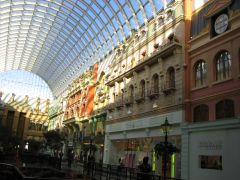
\includegraphics[width=.45\linewidth]{gfx/example_1}} \quad
        \subfloat[Pan ma signo.]
        {\label{fig:example-b}%
         
\includegraphics[width=.45\linewidth]{gfx/example_2}} \\
        \subfloat[Methodicamente o uno.]
        {
\includegraphics[width=.45\linewidth]{gfx/example_3}} \quad
        \subfloat[Titulo debitas.]
        {
\includegraphics[width=.45\linewidth]{gfx/example_4}}
        \caption[Tu duo titulo debitas latente]{Tu duo titulo debitas
        latente.}\label{fig:example}
\end{figure}


%************************************************
\chapter{Math Test Chapter}\label{ch:mathtest} % $\mathbb{ZNR}$
%************************************************
Ei choro aeterno antiopam mea, labitur bonorum pri no. His no decore
nemore graecis. In eos meis nominavi, liber soluta vim cu. Sea commune
suavitate interpretaris eu, vix eu libris efficiantur.

\section{Some Formulas}
Due to the statistical nature of ionisation energy loss, large
fluctuations can occur in the amount of energy deposited by a particle
traversing an absorber element\footnote{Examples taken from Walter
Schmidt's great gallery: \\
\url{http://home.vrweb.de/~was/mathfonts.html}}.  Continuous processes
such as multiple
scattering and energy loss play a relevant role in the longitudinal
and lateral development of electromagnetic and hadronic
showers, and in the case of sampling calorimeters the
measured resolution can be significantly affected by such fluctuations
in their active layers.  The description of ionisation fluctuations is
characterised by the significance parameter $\kappa$, which is
proportional to the ratio of mean energy loss to the maximum allowed
energy transfer in a single collision with an atomic electron:

\[
\kappa =\frac{\xi}{E_{\mathrm{max}}} \mathbb{ZNR}
\]
$E_{\mathrm{max}}$ is the maximum transferable energy in a single
collision with
an atomic electron.
\[
E_{\mathrm{max}} =\frac{2 m_{\mathrm{e}} \beta^2\gamma^2 }{1 +
2\gamma m_{\mathrm{e}}/m_{\mathrm{x}} + \left ( m_{\mathrm{e}}
/m_{\mathrm{x}}\right)^2}\ ,
\]
where $\gamma = E/m_{\mathrm{x}}$, $E$ is energy and
$m_{\mathrm{x}}$ the mass of the incident particle,
$\beta^2 = 1 - 1/\gamma^2$ and $m_{\mathrm{e}}$ is the electron mass.
$\xi$ comes from the Rutherford scattering cross section
and is defined as:
\begin{eqnarray*} \xi  = \frac{2\pi z^2 e^4 N_{\mathrm{Av}} Z \rho
\delta x}{m_{\mathrm{e}} \beta^2 c^2 A} =  153.4 \frac{z^2}{\beta^2}
\frac{Z}{A}
  \rho \delta x \quad\mathrm{keV},
\end{eqnarray*}
where

\begin{tabular}{ll}
$z$          & charge of the incident particle \\
$N_{\mathrm{Av}}$     & Avogadro's number \\
$Z$          & atomic number of the material \\
$A$          & atomic weight of the material \\
$\rho$       & density \\
$ \delta x$  & thickness of the material \\
\end{tabular}

$\kappa$ measures the contribution of the collisions with energy
transfer close to $E_{\mathrm{max}}$.  For a given absorber, $\kappa$
tends
towards large values if $\delta x$ is large and/or if $\beta$ is
small.  Likewise, $\kappa$ tends towards zero if $\delta x $ is small
and/or if $\beta$ approaches $1$.

The value of $\kappa$ distinguishes two regimes which occur in the
description of ionisation fluctuations:

\begin{enumerate}
\item A large number of collisions involving the loss of all or most
  of the incident particle energy during the traversal of an absorber.

  As the total energy transfer is composed of a multitude of small
  energy losses, we can apply the central limit theorem and describe
  the fluctuations by a Gaussian distribution.  This case is
  applicable to non-relativistic particles and is described by the
  inequality $\kappa > 10 $ (when the mean energy loss in the
  absorber is greater than the maximum energy transfer in a single
  collision).

\item Particles traversing thin counters and incident electrons under
  any conditions.

  The relevant inequalities and distributions are $ 0.01 < \kappa < 10
  $,
  Vavilov distribution, and $\kappa < 0.01 $, Landau distribution.
\end{enumerate}


\section{Various Mathematical Examples}
If $n > 2$, the identity
\[
  t[u_1,\dots,u_n] = t\bigl[t[u_1,\dots,u_{n_1}], t[u_2,\dots,u_n]
  \bigr]
\]
defines $t[u_1,\dots,u_n]$ recursively, and it can be shown that the
alternative definition
\[
  t[u_1,\dots,u_n] = t\bigl[t[u_1,u_2],\dots,t[u_{n-1},u_n]\bigr]
\]
gives the same result.


%*****************************************
%*****************************************
%*****************************************
%*****************************************
%*****************************************